\subsection{Pre-trained Text Encoders}
\label{sec:frozen_text_encoders}
We explore several families of pre-trained text encoders: BERT \cite{devlin-naacl-2019}, T5 \cite{raffel-jmlr-2020}, and CLIP \cite{radford-icml-2021}. 
There are several key differences between these encoders. BERT is trained on a smaller text-only corpus (approximately 20 GB, Wikipedia and BooksCorpus \cite{zhu-iccv-2015}) with a masking objective, and has relatively small model variants (upto 340M parameters). T5 is trained on a much larger C4 text-only corpus (approximately 800 GB) with a denoising objective, and has larger model variants (up to 11B parameters). The CLIP model\footnote{\url{https://github.com/openai/CLIP/blob/main/model-card.md}} is trained on an image-text corpus with an image-text contrastive objective. For T5 we use the encoder part for the contextual embeddings. For CLIP, we use the penultimate layer of the text encoder to get contextual embeddings. Note that we freeze the weights of these text encoders (i.e., we use off the shelf text encoders, without any fine-tuning on the text-to-image generation task). We explore a variety of model sizes for these text encoders.

We train a $64\times64$, 300M parameter diffusion model, conditioned on the text embeddings generated from BERT (base, and large), T5 (small, base, large, XL, and XXL), and CLIP (ViT-L/14). We observe that scaling the size of the language model text encoders generally results in better image-text alignment as captured by the CLIP score as a function of number of training steps (see \cref{Fig:EmbeddingTrainingCurves}).
One can see that the best CLIP scores are obtained with the T5-XXL text encoder. 

Since guidance weights are used to control image quality and text alignment, we also report ablation results using curves that show the trade-off between CLIP and FID scores as a function of the guidance weights (see \cref{fig:embedding_comparison_pareto}). We observe that larger variants of T5 encoder results in both better image-text alignment, and image fidelity. This emphasizes the effectiveness of large frozen text encoders for text-to-image models. Interestingly, we also observe that the T5-XXL encoder is on-par with the CLIP encoder when measured with CLIP and FID-10K on MS-COCO.

\textbf{T5-XXL vs CLIP on DrawBench}: We further compare T5-XXL and CLIP on \benchmarkname to perform a more comprehensive comparison of the abilities of these two text encoders. In our initial evaluations we observed that the 300M parameter models significantly underperformed on \benchmarkname. We believe this is primarily because \benchmarkname prompts are considerably more difficult than MS-COCO prompts. 

In order to perform a meaningful comparison, we train 64$\times$64 1B parameter diffusion models with T5-XXL and CLIP text encoders for this evaluation. \cref{fig:drawit_t5_vs_clip} shows the results. We find that raters are considerably more likely to prefer the generations from the model trained with the T5-XXL encoder over the CLIP text encoder, especially for image-text alignment. This indicates that language models are better than text encoders trained on image-text contrastive objectives in encoding complex and compositional text prompts. 
\cref{fig:t5xx_vs_clip_drawbench_details} shows the category specific comparison between the two models. We observe that human raters prefer T5-XXL samples over CLIP samples in all 11 categories for image-text alignment  demonstrating the effectiveness of large language models as text encoders for text to image generation.  

\begin{figure}[t]
    \centering
    \begin{subfigure}[t]{0.49\textwidth}
    \input{figures/pgfplots/encoder_pareto_comparison_appendix}
    \caption{Pareto curves comparing various text encoders.}
     \label{fig:embedding_comparison_pareto}
    \end{subfigure}\hfill
    \begin{subfigure}[t]{0.49\textwidth}
     \centering
     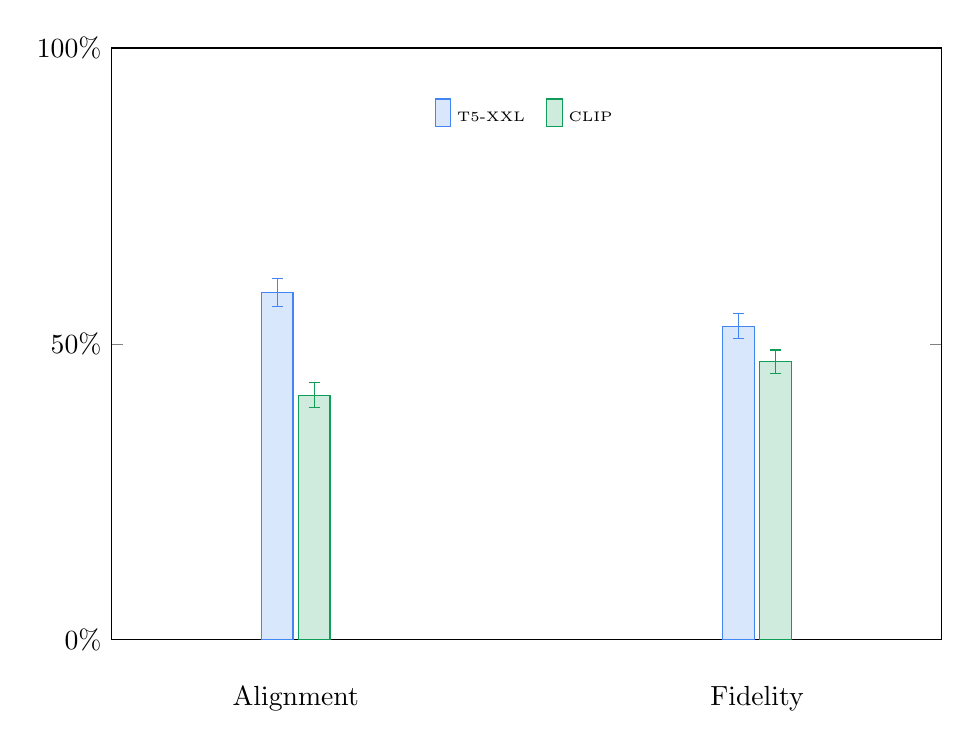
\begin{tikzpicture}

\definecolor{google_blue}{RGB}{66,133,244}
\definecolor{google_red}{RGB}{219,68,55}
\definecolor{google_yellow}{RGB}{194,144,0}
\definecolor{google_green}{RGB}{15,157,88}

\begin{axis}[
name=fidelity,
width=\textwidth,
height=0.75\textwidth,
ybar,
ymin=0.0,
ymax=1.0,
xtick={1, 2},
xtick style={draw=none},
xticklabels={Alignment, Fidelity},
xticklabel style={yshift=-9pt},
ytick={0,0.5,1},
yticklabels={0\%, 50\%, 100\%},
legend style={font=\tiny},
legend cell align=left,
legend image code/.code={
    \draw [#1] (0cm, -0.1cm) rectangle (0.2cm, 0.25cm);
},
legend style={
draw=none,
at={(0.5, 0.925)}, anchor=north,
legend columns=3,
/tikz/every even column/.append style={column sep=0.2cm}
},
bar width=0.4cm,
enlarge x limits={abs=0.4},
]

\addplot+[
    fill=google_blue,
    fill opacity=0.2,
    draw=google_blue,
    error bars/error bar style={google_blue},
    error bars/.cd,
    y dir=both,
    y explicit
] coordinates {
(1.0,0.5867) +- (1.0, 0.02300842393320771)
(2.0,0.530) +- (2.0, 0.02074325857730084)
};
\addplot+[
fill=google_green,fill opacity=0.2,draw=google_green,
    error bars/error bar style={google_green},
    error bars/.cd,
    y dir=both,
    y explicit
] coordinates {
(1.0,0.4133) +- (1.0, 0.02158669186220008)
(2.0,0.470) +- (2.0, 0.019597550393515743)
};


\legend{T5-XXL, CLIP}
\end{axis}
\end{tikzpicture}
      \caption{Comparing T5-XXL and CLIP on \benchmarkname.}
      \label{fig:drawit_t5_vs_clip}
    \end{subfigure}
    \caption{Comparison between text encoders for text-to-image generation. For \cref{fig:embedding_comparison_pareto}, we sweep over guidance values of $[1, 1.25, 1.5, 1.75, 2, 3, 4, 5, 6, 7, 8, 9, 10]$}
\end{figure}

\begin{figure}[t]
    \centering
    \begin{tikzpicture}

\definecolor{google_blue}{RGB}{66,133,244}
\definecolor{google_red}{RGB}{219,68,55}
\definecolor{google_yellow}{RGB}{194,144,0}
\definecolor{google_green}{RGB}{15,157,88}


\begin{axis}[width=10cm, height=5cm,
  xlabel=Training Steps,
  ylabel=CLIP Score,
  legend columns=4,
  legend pos=south east,
  legend style={font=\tiny},
  legend cell align=left,
  xmin=0,
  ymin=0.22,
  xmax=500000,
  every axis plot/.append style={thick}
]
\addplot +[mark=none, dashed, google_blue] table [x=Step, y=Clip Score, col sep=comma] {embedding_comparison/bert_base.csv};
\addplot +[mark=none, dashed, google_red] table [x=Step, y=Clip Score, col sep=comma] {embedding_comparison/bert_large.csv};

\addplot +[mark=none, solid, google_yellow] table [x=Step, y=Clip Score, col sep=comma] {embedding_comparison/t5_small.csv};
\addplot +[mark=none, solid, google_blue] table [x=Step, y=Clip Score, col sep=comma] {embedding_comparison/t5_base.csv};
\addplot +[mark=none, solid, google_red] table [x=Step, y=Clip Score, col sep=comma] {embedding_comparison/t5_large.csv};
\addplot +[mark=none, solid, google_green] table [x=Step, y=Clip Score, col sep=comma] {embedding_comparison/t5_xl.csv};
\addplot +[mark=none, solid, gray] table [x=Step, y=Clip Score, col sep=comma] {embedding_comparison/t5_xxl.csv};
\addplot +[mark=none, dotted] table [x=Step, y=Clip Score, col sep=comma] {embedding_comparison/clip.csv};
\addplot[mark=none, dashdotted] coordinates {(0,0.27089) (1e6,0.27089)};
\legend{BERT Base, BERT Large, T5 Small, T5 Base, T5 Large, T5 XL, T5 XXL, CLIP, Reference}
\end{axis}
\end{tikzpicture}
    \caption{Training convergence comparison between text encoders for text-to-image generation.}
    \label{Fig:EmbeddingTrainingCurves}
\end{figure}


\begin{figure}
    \centering
    \begin{subfigure}[t]{\textwidth}
    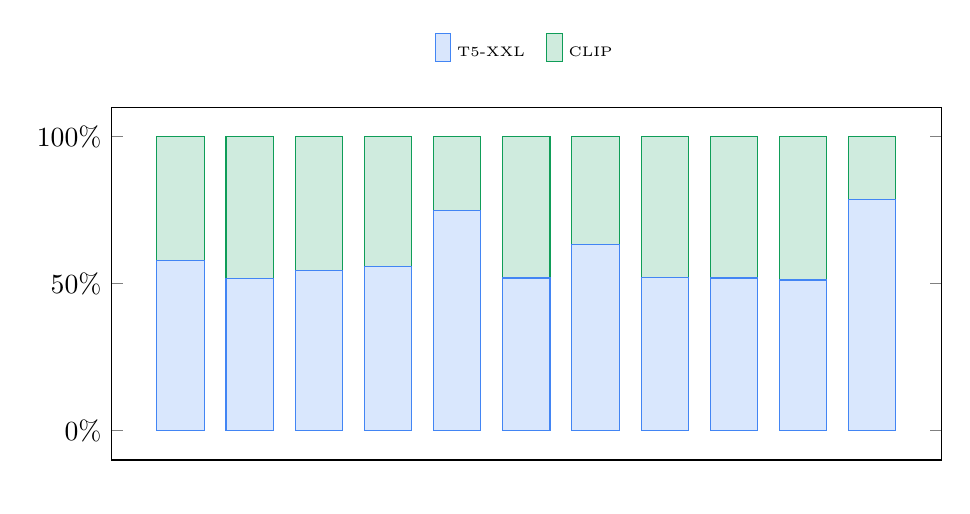
\begin{tikzpicture}

\definecolor{google_blue}{RGB}{66,133,244}
\definecolor{google_red}{RGB}{219,68,55}
\definecolor{google_yellow}{RGB}{194,144,0}
\definecolor{google_green}{RGB}{15,157,88}

\begin{axis}[
name=fidelity,
width=\textwidth,
height=0.5\textwidth,
ybar stacked,
ymin=-0.1,
ymax=1.1,
xtick=data,
xtick style={draw=none},
symbolic x coords={Colors,Conflicting,Counting,DALL-E \cite{ramesh-dalle},Descriptions,Marcus et al. \cite{marcus-arxiv-2022},Misspellings,Positional,Rare Words,Reddit,Text},
xticklabels={},
x tick label style={rotate=30},
ytick={0,0.5,1},
yticklabels={0\%, 50\%, 100\%},
legend style={font=\tiny},
legend cell align=left,
legend image code/.code={
    \draw [#1] (0cm, -0.1cm) rectangle (0.2cm, 0.25cm);
},
legend style={
draw=none,
at={(0.5, 1.1)},anchor=south,
legend columns=3,
/tikz/every even column/.append style={column sep=0.2cm}
},
bar width=0.6cm,
]

\addplot+[
    fill=google_blue,
    fill opacity=0.2,
    draw=google_blue
] coordinates {
(Colors, 0.579)
(Conflicting, 0.517)
(Counting, 0.543)
(DALL-E \cite{ramesh-dalle}, 0.559)
(Descriptions, 0.749)
(Marcus et al. \cite{marcus-arxiv-2022}, 0.519)
(Misspellings, 0.632)
(Positional, 0.522)
(Rare Words, 0.519)
(Reddit, 0.512)
(Text, 0.785)
};

\addplot+[
fill=google_green,
fill opacity=0.2,
draw=google_green
] coordinates {
(Colors, 0.421)
(Conflicting, 0.483)
(Counting, 0.456)
(DALL-E \cite{ramesh-dalle}, 0.441)
(Descriptions, 0.251)
(Marcus et al. \cite{marcus-arxiv-2022}, 0.481)
(Misspellings, 0.368)
(Positional, 0.478)
(Rare Words, 0.481)
(Reddit, 0.488)
(Text, 0.214)
};

\legend{T5-XXL, CLIP}
\end{axis}

\end{tikzpicture}
    \caption{Alignment}
    \label{fig:t5xxl_vs_clip_detailed_alignment_alignment}
    \vspace*{0.5cm}
    \end{subfigure}
    \begin{subfigure}[t]{\textwidth}
    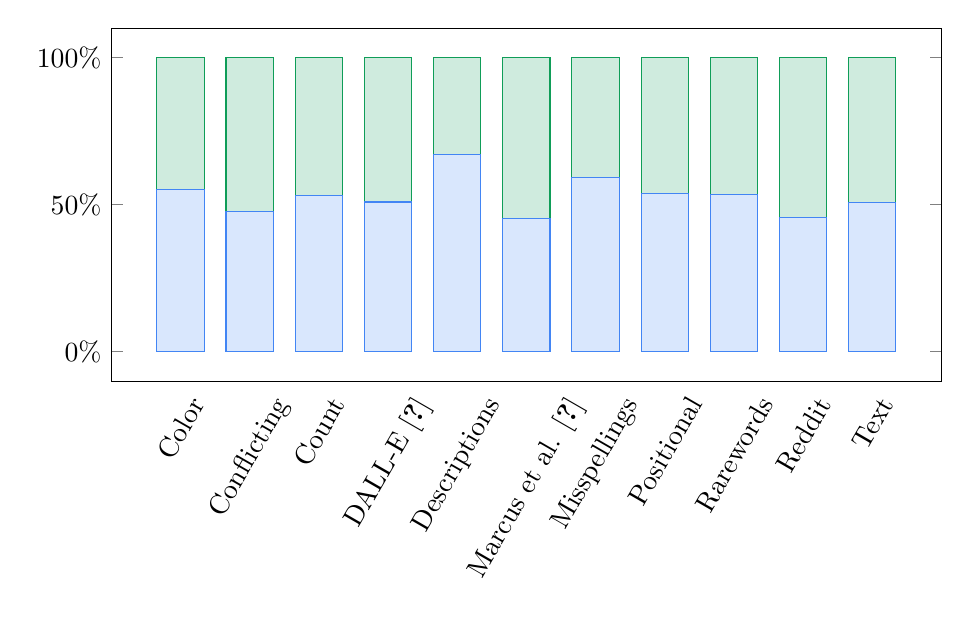
\begin{tikzpicture}

\definecolor{google_blue}{RGB}{66,133,244}
\definecolor{google_red}{RGB}{219,68,55}
\definecolor{google_yellow}{RGB}{194,144,0}
\definecolor{google_green}{RGB}{15,157,88}

\begin{axis}[
name=fidelity,
width=\textwidth,
height=0.5\textwidth,
ybar stacked,
ymin=-0.1,
ymax=1.1,
xtick=data,
xtick style={draw=none},
symbolic x coords={Color,Conflicting,Count,DALL-E \cite{ramesh-dalle},Descriptions,Marcus et al. \cite{marcus-arxiv-2022},Misspellings,Positional,Rarewords,Reddit,Text},
x tick label style={rotate=60},
ytick={0,0.5,1},
yticklabels={0\%, 50\%, 100\%},
legend style={font=\tiny},
legend cell align=left,
legend image code/.code={
    \draw [#1] (0cm, -0.1cm) rectangle (0.2cm, 0.25cm);
},
legend style={
draw=none,
at={(0.5, 1.1)},anchor=south,
legend columns=3,
/tikz/every even column/.append style={column sep=0.2cm}
},
bar width=0.6cm,
]
\addplot+[
    fill=google_blue,
    fill opacity=0.2,
    draw=google_blue
] coordinates {
(Color, 0.552)
(Conflicting, 0.476)
(Count, 0.532)
(DALL-E \cite{ramesh-dalle}, 0.509)
(Descriptions, 0.671)
(Marcus et al. \cite{marcus-arxiv-2022}, 0.453)
(Misspellings, 0.591)
(Positional, 0.538)
(Rarewords, 0.536)
(Reddit, 0.457)
(Text, 0.507)
};

\addplot+[
fill=google_green,
fill opacity=0.2,
draw=google_green
] coordinates {
(Color, 0.448)
(Conflicting, 0.524)
(Count, 0.468)
(DALL-E \cite{ramesh-dalle}, 0.491)
(Descriptions, 0.329)
(Marcus et al. \cite{marcus-arxiv-2022}, 0.547)
(Misspellings, 0.409)
(Positional, 0.462)
(Rarewords, 0.464)
(Reddit, 0.543)
(Text, 0.493)
};


\legend{}
\end{axis}
\end{tikzpicture}
    \caption{Fidelity}
    \label{fig:t5xxl_vs_clip_detailed_alignment_fidelity}
    \end{subfigure}
    \caption{T5-XXL vs. CLIP text encoder on \benchmarkname \subref{fig:t5xxl_vs_clip_detailed_alignment_alignment}) image-text alignment, and \subref{fig:t5xxl_vs_clip_detailed_alignment_fidelity}) image fidelity.}
    \label{fig:t5xx_vs_clip_drawbench_details}
\end{figure}

